\chapter{Implementação e preparação do ambiente}
\label{cap:implementacao}

Este capítulo apresenta a passagem da hipótese arquitetural para a implementação utilizada nos ensaios. A contribuição prática compreende a adaptação do núcleo Python, a definição das fronteiras de estado e comunicação e a construção de bancadas em Docker e Kubernetes. O protocolo de medição, descrito no Capítulo~\ref{cap:metodologia-tcc2}, utiliza essa implementação sem substituir a validação funcional pela simples observação de respostas HTTP.

\section{Código de referência e delimitação da adaptação}

O ponto de partida foi o código Python fornecido no contexto da orientação e disponibilizado no repositório \texttt{JnetSilvestre/codigoPon}, na revisão \texttt{c2d525b5c675}. Essa referência foi fixada para permitir distinguir o material recebido das alterações realizadas neste trabalho. Os arquivos usados nas Listagens~\ref{lst:atributo-original} e~\ref{lst:composicao-original} foram conferidos diretamente nessa revisão e acompanham o projeto em \texttt{uteis/codigo-original}. A referência bibliográfica identifica a versão consultada \cite{codigoponreferencia}.

Essa implementação representa entidades do PON em Python. Embora a motivação do estudo se relacione à linha de pesquisa sobre NOP Query, a aplicação ensaiada não implementa o sistema completo de consultas em vídeo em C++ descrito por \citeonline{kossoski2024tese}. O objeto experimental é a cadeia de atributos, premissas, condições, regras e ações da prova de conceito. Essa delimitação evita atribuir ao sistema original resultados medidos em uma adaptação menor e com outro ambiente de execução.

\subsection{Notificação de mudanças e composição lógica}

A Listagem~\ref{lst:atributo-original} mostra o mecanismo original de atualização de um atributo. A comparação entre o valor anterior e o recebido precede a chamada de atualização. Assim, uma atribuição que mantém o mesmo valor não percorre a cadeia de notificações por esse caminho. Essa distinção foi mantida na adaptação e tornou-se observável nos registros de operações sem alteração, denominadas \textit{no-ops}.

\begin{sourcecode}[htbp]
\caption{Trecho original: atualização de valor em \texttt{Attribute}.}
\label{lst:atributo-original}
\lstinputlisting[style=tccpython,firstline=17,lastline=23,firstnumber=17]{uteis/codigo-original/Attribute.py}
\fonte{Código de referência, revisão \texttt{c2d525b5c675}, \texttt{pon/Attribute.py}}
\end{sourcecode}

A composição de condições também está presente no código recebido. Na Listagem~\ref{lst:composicao-original}, a operação lógica E cria uma condição associada aos dois elementos de entrada. O registro das dependências permite que mudanças sejam propagadas entre entidades. O uso de operadores da linguagem facilita a expressão da regra, mas não acrescenta transporte entre processos: as referências aos elementos continuam sendo objetos locais.

\begin{sourcecode}[htbp]
\caption{Trecho original: composição de condições pela operação lógica E.}
\label{lst:composicao-original}
\lstinputlisting[style=tccpython,firstline=60,lastline=65,firstnumber=60]{uteis/codigo-original/Condition.py}
\fonte{Código de referência, revisão \texttt{c2d525b5c675}, \texttt{pon/Condition.py}}
\end{sourcecode}

\subsection{Ajustes funcionais e referência local}

A preparação da referência local C0 exigiu ajustes identificados na cópia de trabalho. Em \texttt{Condition.update}, a propagação passou a notificar os observadores da condição; o identificador herdado passou a ser acessado por \texttt{getId()}. Em \texttt{Rule}, o caminho de notificação passou a executar a ação sincronamente, sem depender de agendamento implícito em um laço assíncrono. O cadastro de entidades também recebeu verificações de colisão e propriedade de identificadores. Essas mudanças estão documentadas no histórico da implementação e não foram aplicadas ao repositório de referência.

A distinção é relevante para interpretar a contribuição: a versão recebida fornece a estrutura das entidades, enquanto o TCC2 estabelece um caminho funcional determinístico e os mecanismos necessários para atravessar fronteiras de processo. Os testes da referência local verificaram transições da condição, acionamento da regra e ausência de notificações redundantes nos casos definidos. A validação foi complementada por um oráculo que calcula os resultados a partir das entradas sem importar o núcleo PON.

No cenário experimental, a condição avaliada foi
\begin{equation}
 C = (\mathrm{atA} \geq 5) \land (\mathrm{atB}=1).
\label{eq:condicao-experimental}
\end{equation}
Os atributos iniciam com valor zero. Uma transição de $C$ para verdadeiro produz um efeito; a transição para falso atualiza o estado sem disparar a ação. Permanecer em verdadeiro também não representa um novo disparo. O exemplo mínimo de sete passos e a carga de 1.000 operações exercitam essa semântica, com finalidades distintas: o primeiro facilita a inspeção funcional e a segunda compõe a campanha temporal.

\section{Separação em três serviços}
\label{sec:implementacao-servicos}

A Figura~\ref{fig:arquitetura-implementada} apresenta a divisão efetivamente implementada. As entidades logicamente relacionadas permanecem agrupadas no mesmo processo quando sua interação não precisa atravessar a rede. A escolha de três serviços evita transformar cada objeto PON em um Pod e mantém explícitas as duas fronteiras de comunicação investigadas.

\begin{figure}[htbp]
\centering
\caption{Relação entre o núcleo de referência e os serviços implementados.}
\label{fig:arquitetura-implementada}
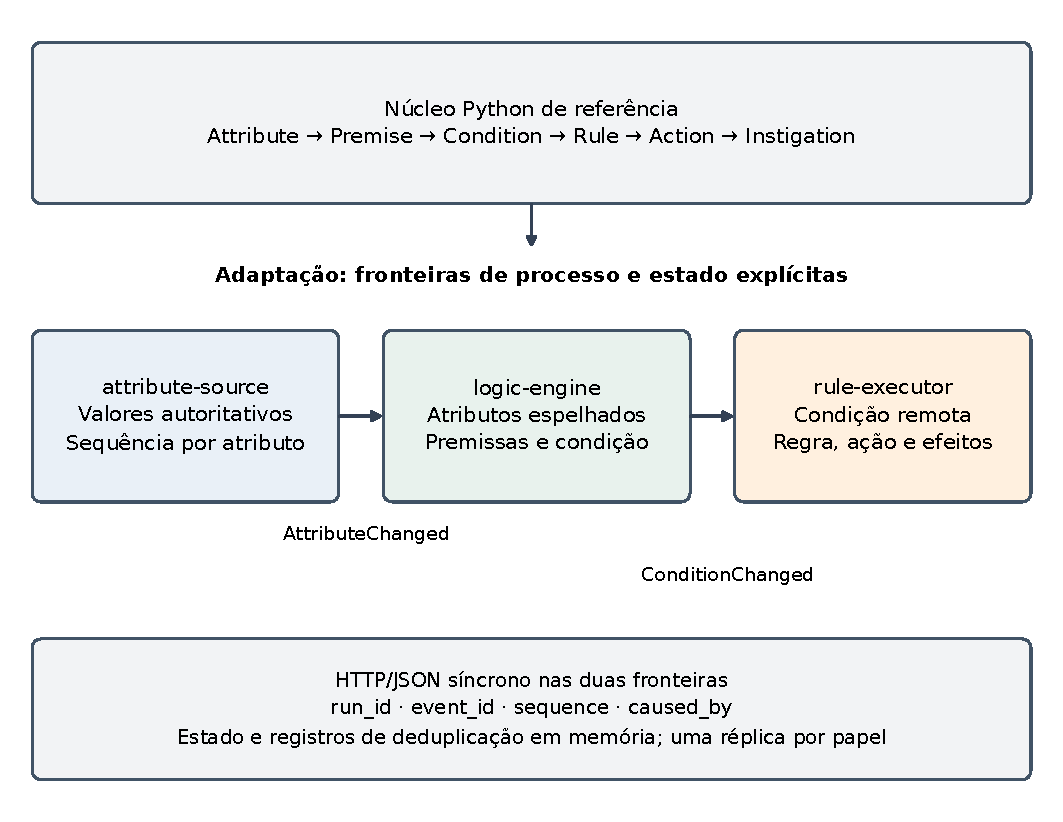
\includegraphics[width=\linewidth]{tcc2-arquitetura-servicos.pdf}
\fonte{}
\end{figure}

O \texttt{attribute-source} é o proprietário dos valores dos atributos. Ele recebe a solicitação do cliente, verifica se houve alteração e atribui uma sequência à mudança efetiva. O \texttt{logic-engine} mantém os atributos espelhados usados na avaliação das premissas e da condição. O \texttt{rule-executor} mantém o estado da condição remota e transforma suas transições em efeitos por meio de regra, ação e instigação locais. Cada papel possui seus próprios registros em memória.

Não se trata de três cópias independentes da aplicação. A execução depende de uma cadeia: o produtor encaminha uma alteração ao avaliador, que pode encaminhar uma transição ao executor. O cliente recebe a resposta depois do retorno das chamadas síncronas pertinentes. Em uma operação sem mudança de atributo, o fluxo termina no produtor; em uma mudança que não altera a condição, não ocorre a segunda notificação. Por isso, as 1.000 requisições não representam 1.000 percursos idênticos pelos três serviços.

A Listagem~\ref{lst:adaptacao-condicao} mostra a conexão do estado recebido com o núcleo local no avaliador. O observador registrado converte uma transição da condição em mensagem para o próximo serviço. Esse trecho pertence à adaptação desenvolvida no TCC2, e não ao código original.

\begin{sourcecode}[htbp]
\caption{Adaptação: construção da cadeia lógica a partir do snapshot.}
\label{lst:adaptacao-condicao}
\lstinputlisting[style=tccpython,firstline=146,lastline=154,firstnumber=146]{uteis/codigo-tcc2/state.py}
\fonte{Implementação do TCC2, \texttt{prova-conceito/c1/state.py}}
\end{sourcecode}

\section{Inicialização, contratos e consistência do estado}

Antes de processar alterações, o produtor instala um \textit{snapshot} com os valores e as sequências iniciais no avaliador. Este constrói a condição local e inicializa o executor com o estado lógico correspondente. O produtor somente registra a inicialização como concluída depois da confirmação do encaminhamento. A Figura~\ref{fig:sequencia-implementada} distingue esse procedimento do caminho de uma mudança que resulta em efeito.

\begin{figure}[htbp]
\centering
\caption{Inicialização e percurso síncrono de uma mudança que produz efeito.}
\label{fig:sequencia-implementada}
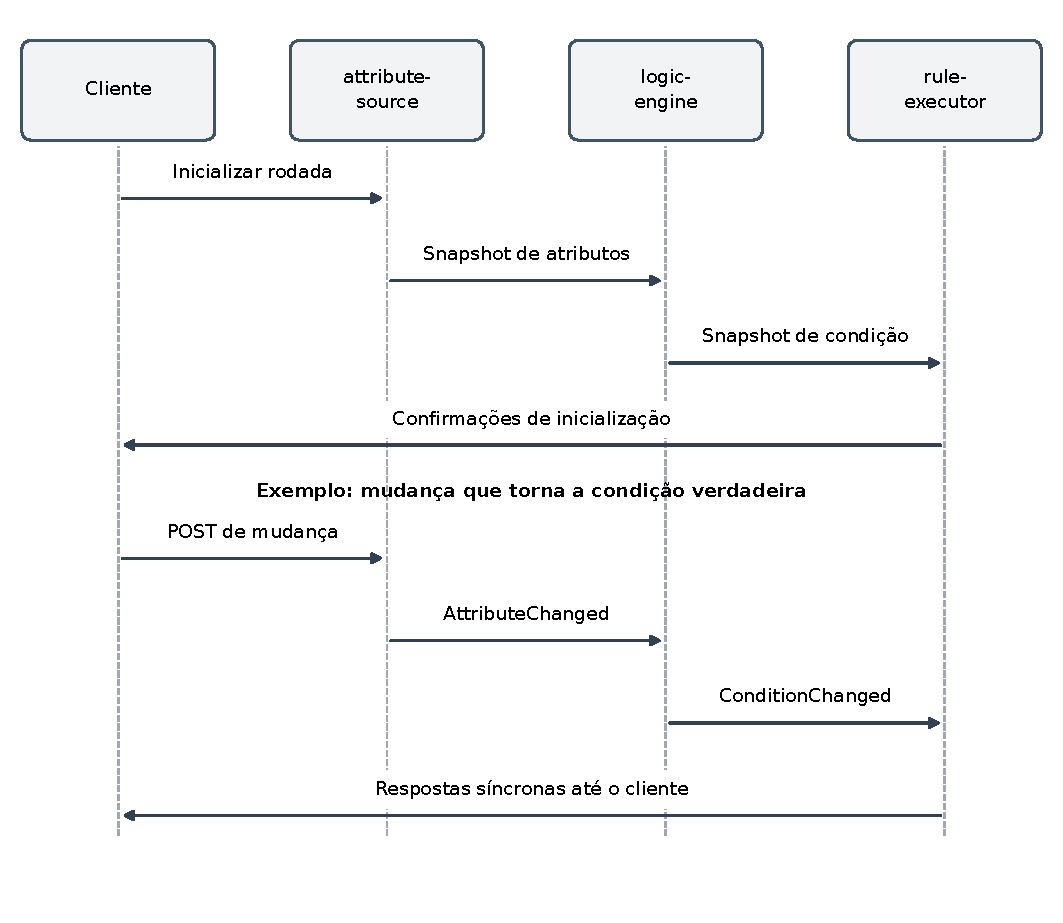
\includegraphics[width=.96\linewidth]{tcc2-sequencia-notificacoes.pdf}
\fonte{}
\end{figure}

As mensagens usam JSON e versão explícita de esquema. Os campos de identidade permitem acompanhar a cadeia sem calcular latências pela subtração de relógios de processos diferentes. A Tabela~\ref{tab:contratos-estado} sintetiza os campos mais relevantes. A expressão \texttt{caused\_by} liga uma transição de condição à mudança de atributo que a provocou e liga o efeito à transição correspondente.

\begin{table}[htbp]
\centering\small
\caption{Identificadores e controles dos contratos de comunicação.}
\label{tab:contratos-estado}
\begin{tabularx}{\linewidth}{@{}p{3.3cm}X@{}}
\toprule
Campo & Função na implementação \\
\midrule
\texttt{schema\_version} & Identificar o formato validado da mensagem. \\
\texttt{run\_id} & Impedir a mistura de mensagens de rodadas distintas. \\
\texttt{request\_id} & Identificar a solicitação do cliente e detectar reutilização conflitante. \\
\texttt{event\_id} & Correlacionar emissão, recepção, deduplicação e efeito. \\
\texttt{entity\_id} e \texttt{sequence} & Identificar a entidade e exigir continuidade de sua sequência. \\
\texttt{caused\_by} & Preservar a relação causal entre mensagens e efeitos. \\
\texttt{snapshot\_version} & Identificar o estado usado na inicialização da rodada. \\
\bottomrule
\end{tabularx}
\fonte{}
\end{table}

Mensagens já registradas com o mesmo conteúdo são reconhecidas como duplicadas; o mesmo identificador com conteúdo diferente é rejeitado. O receptor também rejeita lacunas de sequência e mensagens de outra rodada. Esses controles foram exercitados nos testes funcionais anteriores à campanha, incluindo repetição de mensagens e conflitos de conteúdo. Eles não significam entrega exatamente uma vez sob qualquer falha: os registros de deduplicação são voláteis e não sobrevivem à perda do processo.

Em falha parcial de encaminhamento, o produtor mantém o evento pendente para preservar sua identidade. No avaliador e no executor, uma exceção durante a propagação coloca o estado em falha, evitando presumir um desfazimento de alterações já realizadas. A campanha principal não explorou reinicialização ou recuperação; o controlador interrompe a sequência em erro e não repete automaticamente uma solicitação cujo resultado seja incerto.

\section{Conteinerização e preparação da infraestrutura}

A infraestrutura foi construída de forma incremental. Primeiro, o núcleo foi verificado localmente em C0; em C1, foram introduzidos os processos HTTP; em C2, os serviços passaram a contêineres Docker; em C3 e C4, foram implantados em Kubernetes. Essa progressão permitiu investigar problemas de lógica e contrato antes de acrescentar orquestração e posicionamento entre nós.

O \texttt{Dockerfile} da prova de conceito empacota o código e estabelece o ambiente Python usado pelos processos. A campanha conferiu o identificador da imagem e os limites configurados, em vez de assumir que a igualdade de uma etiqueta de imagem asseguraria conteúdo idêntico. Os serviços e o cliente foram executados na imagem aprovada. O cliente persistente realiza o lote dentro da rede da bancada; não é criado um novo processo \texttt{kubectl exec} para cada POST.

O cluster kind possui um nó de controle e um worker. O arquivo de configuração efetivamente versionado aparece na Listagem~\ref{lst:kind-config}. A documentação do kind define seus nós como contêineres usados para executar um cluster local \cite{kinddocumentation}. A Figura~\ref{fig:camadas-ambiente} explicita as camadas presentes no experimento: os dois nós virtuais compartilham o mesmo equipamento e a infraestrutura WSL2/Docker Desktop.

\begin{sourcecode}[htbp]
\caption{Configuração dos dois nós virtuais do cluster kind.}
\label{lst:kind-config}
\lstinputlisting[style=tcccode,firstline=3]{uteis/codigo-tcc2/kind-config.yaml}
\fonte{Configuração versionada em \texttt{infraestrutura/kind/kind-config.yaml}}
\end{sourcecode}

\begin{figure}[htbp]
\centering
\caption{Camadas de execução e compartilhamento do host físico.}
\label{fig:camadas-ambiente}
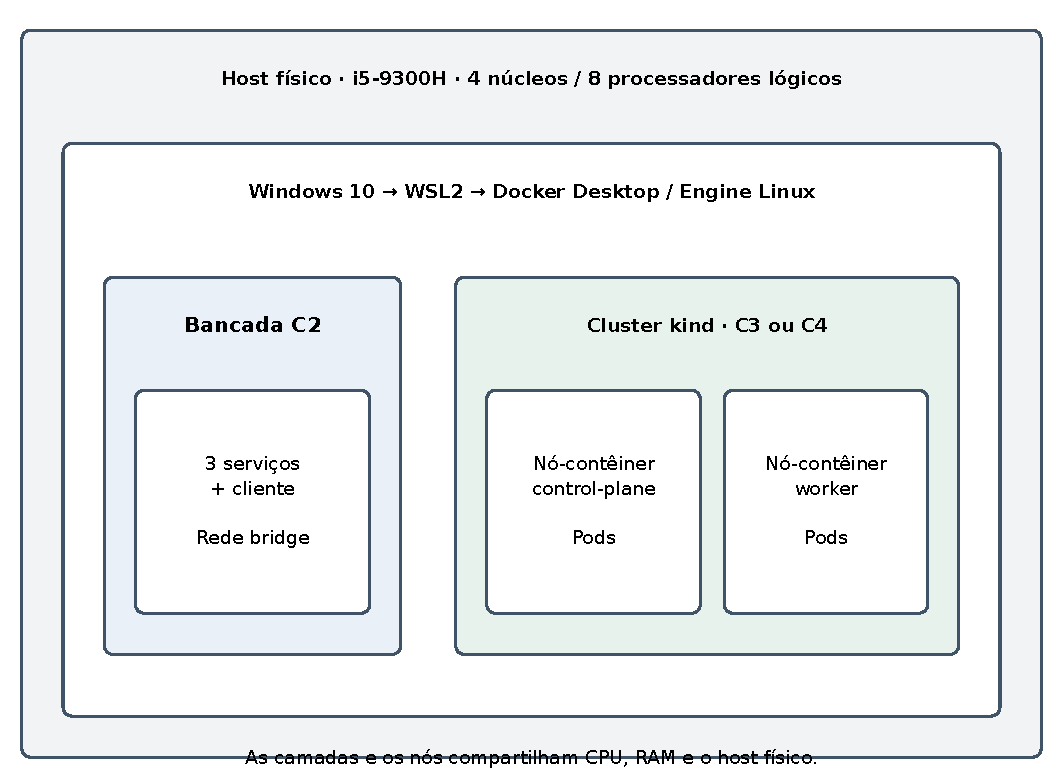
\includegraphics[width=\linewidth]{tcc2-camadas-ambiente.pdf}
\fonte{}
\end{figure}

Cada cenário Kubernetes utiliza um namespace próprio por rodada, três Deployments com uma réplica e três Services internos. A configuração dos destinos da cadeia é fornecida por ConfigMap. Seletores de nó definem o posicionamento requerido. As verificações confrontam a intenção declarada nos manifestos com os Pods observados, seus identificadores e o nó de execução. O Apêndice~\ref{ap:rastreabilidade} indica os arquivos e as revisões que permitem inspecionar essas decisões.

\section{Topologias efetivamente avaliadas}
\label{sec:topologias}

A Figura~\ref{fig:topologias} compara as três configurações da campanha. Em C2, os três serviços e o cliente são contêineres ligados a uma rede bridge interna. Em C3, os três Pods de serviço e o cliente estão no worker. Em C4, o avaliador lógico é colocado no control-plane, enquanto produtor, executor e cliente permanecem no worker. Nesse último caso, as duas fronteiras de notificação atravessam nós virtuais.

\begin{figure}[htbp]
\centering
\caption{Posicionamento dos componentes em C2, C3 e C4.}
\label{fig:topologias}
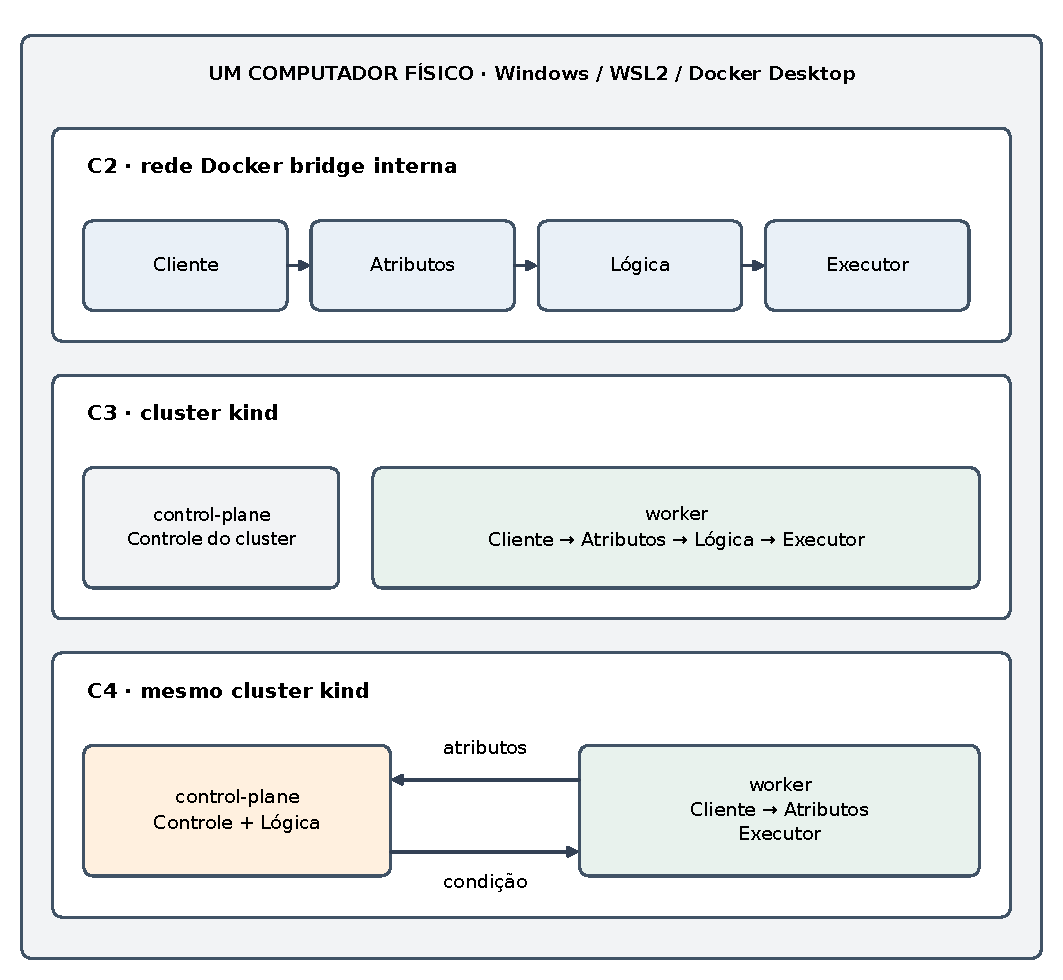
\includegraphics[width=.97\linewidth]{tcc2-topologias-c2-c3-c4.pdf}
\fonte{}
\end{figure}

O posicionamento em C4 demonstra que a cadeia pode atravessar a rede interna entre nós kind preservando o comportamento observado. Entretanto, o control-plane também executa componentes de controle. Portanto, C3 e C4 diferem tanto no percurso de comunicação quanto no contexto de execução do avaliador. Essa configuração não permite atribuir toda diferença de tempo exclusivamente ao tráfego entre nós.

A opção por uma réplica de cada papel mantém um único proprietário para cada estado. Aumentar réplicas sem definir particionamento, roteamento e recuperação poderia enviar mensagens de uma mesma entidade a instâncias com históricos diferentes. Assim, os mecanismos de implantação do Kubernetes foram utilizados para organizar e posicionar a aplicação; escalabilidade horizontal e tolerância a falhas permanecem questões para extensões com protocolos próprios.
